\documentclass[a4paper]{article}

\usepackage[english]{babel}
\usepackage[utf8]{inputenc}
\usepackage{amsmath}
\usepackage{graphicx}
\usepackage[colorinlistoftodos]{todonotes}
\usepackage{fullpage}
\usepackage{graphicx}
\usepackage{caption}
\usepackage{subcaption}
\usepackage{amssymb}
\usepackage{float}
\usepackage{multicol}
\usepackage{geometry}
 \geometry{
 a4paper,
 left=20mm,
 right=20mm,
 % For multicol
 % left=15mm,
 % right=15mm, 
 top=20mm,
 bottom=20mm,
 }

\title{UCLA Computer Science Master's Comprehensive Exam: Implementation and Extension of Followship-LDA}

\author{Spencer Tung \\ Advisor: Professor Junghoo Cho}

\date{\today}

\begin{document}
\maketitle
% \begin{multicols}{2}

%%%%%%%%%%%%%%%%%%%%%%%%%%%%%%%%%%%% Abstract%%%%%%%%%%%%%%%%%%%%%%%%%%%%%%%%%%
\begin{abstract}
asdf
\end{abstract}

%%%%%%%%%%%%%%%%%%%%%%%%%%%%%%%%%%%% Section 1: Project Idea%%%%%%%%%%%%%%%%%%%%%%%%%%%%%%%%%%
\section{Introduction}
Semantic analysis, the art of getting computers and programs to understand the meaning behind text, has been a long standing problem in computer science. There can be many practical applications of semantic analysis, such as identifying the topics that comprise a given document. This, in turn, could be used to determine what sort of topics the reader of this document is potentially be interested in. In today's advertisement-driven and consumer-focused world, being able to automatically obtain this information, independent of the source, is invaluable.

These days, there is a large amount of traffic centered around social media, which many advertisers leverage to market their products. Twitter is one such social media site, focused on microblogs of 140 characters or less. Every time a Twitter user submits a post, known as a \textit{tweet}, the tweet is blasted out to all of the other users that have chosen to \textit{follow} this specific user. The information flow is therefore generated by the \textit{followee} and received by the \textit{follower}. On a microblog site such as Twitter, it can be difficult for marketers to determine where their ads will have the most weight, as there are literally millions of tweets coming from millions of users every day \cite{TODO}. Knowing who key influencers are on Twitter goes a long way for advertisers, who can be more selective about how they reach out to their audience.

However, there are some advertisers who, instead of taking the time to do their own research and fine tune their efforts, will resort to more widespread methods to attract followers. This will often take the form of a computer scipt that blasts their advertisements to anyone who follows them. Known as \textit{Twitterbots}, or spambots to most, these drones are often viewed as being annoyances to legitimate users who may not care for the bot tweets. It is therefore advantageous to be able to automatically identify whether a user is legitimate or a bot and take appropriate measures accordingly.

This paper will focus on an extension of \textit{Latent Dirichlet Analysis} (LDA). LDA is a probabilistic topic model, and can be applied to a set of documents (known as a \textit{corpus}) to extract topic information for each document and every word in a given corpus. The extension of this model, known as \textit{Followship-LDA} (FLDA), leverages Twitter follower-followee network information to identify either important and influential entities on Twitter, or spambots that most people won't pay attention to and should remove from their followee list. The details of both models will be discussed in Section \ref{sec:prevwork}.

The paper will be organized as follows. Section \ref{sec:prevwork} will discuss any previous work that came before this paper. Most importantly, it details the FLDA method critical to algorithm's success. Section \ref{sec:approach} will discuss the system architecture and design. Section \ref{sec:results} will detail the results of running the FLDA model on the Twitter data subset. Finally, Section \ref{sec:conc} will discuss the conclusions.

% \subsection{Motivation}
% I chose this project to further my understanding of semantic analysis, as well as challenge myself by implementing an algorithm that could efficiently deal with big data.


%%%%%%%%%%%%%%%%%%%%%%%% Section 2: Methodology and Previous Work%%%%%%%%%%%%%%%%%%%%%%%%%%%
\section{Background and Previous Work}
\label{sec:prevwork}
\subsection{Background Overview}
To understand how FLDA works, it is necessary to first gain an understanding of how LDA works. As mentioned previously, LDA is a type of probabilistic topic model, which is one approach for semantic analysis. These are models that operate under the following assumptions: that a document is a mixture of different topics, and each topic is a distribution of words. As these are \textit{generative models} for documents, it demonstrates a probabilistic procedure that can be used to generate various documents. Table \ref{tab:ldatopics} shows two example topics, ranked by top 4 words that have a high probability of belonging to that topic. Note that although neither topic is labeled, it is clear to see that Topic 1 most likely has to do with fictional works, whereas Topic 2 revolves around plants and nature. To generate documents from these topics, one simply assigns a probability to each topic and selects words based on the probability distribution of the words in the topics \cite{lda}. In this example, by assigning an equal probability to both topics in this table, one could generate a document that talked about the fictional story of a tree who wanted a bee to come along and pollinate his flowers.

\begin{table}[h]
  \centering % used for centering table
  \begin{tabular}{ |l|l|l|l|l| }
    \cline{0-1}
    \cline{4-5}
    \multicolumn{2}{|l|}{\textbf{Topic 1}} & & \multicolumn{2}{|l|}{\textbf{Topic 2}} \\
    \cline{0-1}
    \cline{4-5}
    word & prob & & word & prob \\
    \cline{0-1}
    \cline{4-5}
    BOOK & 0.06 & & TREE & 0.04 \\
    NOVEL & 0.04 & & FLOWERS & 0.03 \\
    STORY & 0.03 & & POLLEN & 0.03 \\
    HARDCOVER & 0.01 & & FRUIT & 0.02 \\
    \cline{0-1}
    \cline{4-5}
  \end{tabular}
  \caption{Two inferred topics as a result of running LDA on a given corpus. These topic probabilities can also in turn be used to generate documents by selecting words from each topic.}
  \label{tab:ldatopics}
\end{table}

Using statistical techniques, it is possible to invert this process and infer the set of topics that were used to generate the documents in question. That is, given a set of documents, one could return a list of topics, each with their own probability distribution of likely words. This is the process known as LDA.

\subsection{LDA}
To start, we first define some variables and equations. $P(z)$ is the probability distribution of topics $z$ over a given document - an example of this would be the equal document we generated previously. There, both topics 1 and 2 had a $50\%$ probability of showing up in the document. $P(w | z)$ is the probability of word $w$ being chosen, given topic $z$. This would be represented by the probabilities listed in Table \ref{tab:ldatopics}. More common or otherwise prominent words for a topic $z$ are given higher weights that the less used ones. A document can therefore be generated, word by word, by first selecting a topic from the distribution of topics, and then sampling a word $w_i$ from the topic-word distribution $P(w | z)$. We represent these two actions with $P(z_i = j)$, which is the probability that for the $i$th word token in a given document, the $j$th topic was selected, and $P(w_i | z_i = j)$, which is the probability of word $w_i$ in topic $j$'s word distribution.

We can simplify the notation using $\phi^{(j)}$ to represent this multinomial distribution of the words for topic $j$, and $\theta^{(d)}$ to represent the multinomial distribution of topics for document $d$. In essence, $\phi$ denotes which words are important for a given topic, and $\theta$ will list out the important topics for a given document. Finally, given that we are inferring these document-topic and topic-word distributions with no prior information about the corpus (ie. the set of documents), we must select a total number of topics $T$ for our inference. The total number of documents in our corpus is $D$, where each document $d$ consists of $N_d$ words, and the total number of words is $N$, where $N = \sum\limits^D{N_d}$ \cite{lda}. Table \ref{tab:ldavars} lists out the aforementioned variables for easy reference.
\begin{table}[h]
  \centering % used for centering table
  \begin{tabular}{ |l|l| }
    \hline
    Notation & Description \\
    \hline
    \hline
    $P(z)$ & Distribution of topics $z$ over a given document \\
    $P(w | z)$ & Distribution of words $w$ over a given topic $z$ \\
    $P(z_i = j)$ & Probability that topic $j$ was sampled for the $i$th word in a given document \\
    $P(w_i | z_i = j)$ & Probability of word $w_i$ for topic $j$ \\
    $\phi^{(j)}$ & Simplified representation of $P(w | z = j)$, for topic $j$ \\
    $\theta^{(d)}$ & Simplified representation of $P(z)$, for document $d$ \\
    $w_i$ & $i$th word in a document \\
    $T$ & Number of topics, manually chosen \\
    $D$ & Number of documents in the corpus \\
    $N_d$ & Number of words in document $d$ \\
    $N$ & Number of words in the corpus \\
    \hline
  \end{tabular}
  \caption{Quick reference for notation and variables used in LDA}
  \label{tab:ldavars}
\end{table}

Given the document-topic and topic-word probability distributions, we can subsequently define the probability distribution of each word in a document with $P(w_i)$, in Equation \ref{eq:lda_probdist}.

\begin{equation}\label{eq:lda_probdist}
  P(w_i) = \sum\limits_{j=1}^T P(w_i | z_i = j) P(z_i = j) = (\phi^{(j)}_i) (\theta^{(d)}_i)
\end{equation}

As the number of topics is manually specified by the user, this operation's space and time complexity is constrained by $T$. If we extend the visualization from Table \ref{tab:ldatopics} (simplified as $\phi$), we can imagine $\phi$ as a 2D matrix, with each word token index represented by the row indices $i$, the topic indices represented by the column indices $j$. The entries of this matrix are then the probabilities of word $i$ being assigned to a topic $j$. We use a similar definition to define $\theta$, where the entries of this 2D matrix are the probabilities of topic $i$ being assigned to document $j$. Figure \ref{fig:topicmodel} gives a visual representation of Equation \ref{eq:lda_probdist}. It is clear to see from Figure \ref{fig:topicmodel} that it is important to choose an appropriate value for $T$ in order to have meaningful results for $\theta$ and $\phi$ \cite{lda}.

\begin{figure}[h]
  \centering
    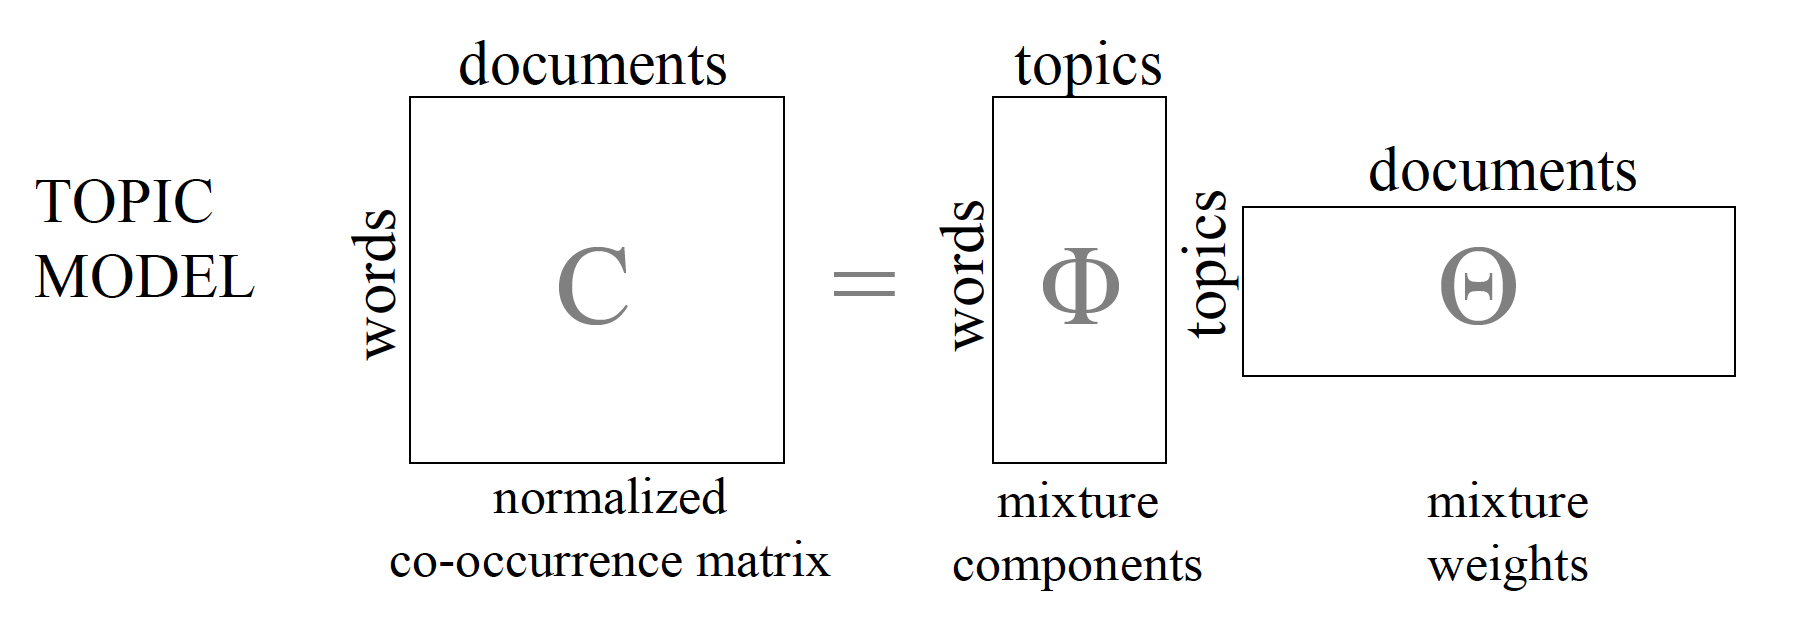
\includegraphics[width=0.7\textwidth]{topicmodel}
  \caption {Visual representation of the probabilistic topic model}
  \label{fig:topicmodel}
\end{figure}

LDA distinguishes itself from other probabilistic topic model by including a \textit{Dirichlet prior} on the $\theta$ parameter. The use of a prior allows for the algorithm to make a general assumption about how its weights are generated, based on the total number of topics chosen \cite{hoffman}. As the Dirichlet distribution is a conjugate prior for the multinomial distribution, this means that the posterior distribution will also be a Dirichlet. In addition, it is relatively simple to sample from the Dirichlet distribution. While a detailed explanation of conjugate priors is outside of the scope of this paper, we will turn our focus instead to the portions that will allow us to implement LDA \cite{lda}. It is sufficient to know that the Dirichlet distribution is used to model the multinomial distribution of $\theta$, and the parameters of the Dirichlet distribution are known as \textit{hyperparameters}, distinguishing them from the parameters $\theta$ and $\phi$ of the underlying distribution. In our situation, each hyperparameter $\alpha_j$ from $\alpha_1, ..., \alpha_T$ represents the initial, prior count for the number of times topic $j$ was sampled in a document. A similar hyperparameter $\beta$ is assigned to model $\phi$ as well, representing the prior count for the number of times a word was sampled from a topic. It is important to remember that this occurs before we have even begun the actual sampling process.

\subsection{Gibbs Sampling}
As mentioned in the previous section, one of the reasons a Dirichlet prior is included is because it is simple to sample from a Dirichlet distribution. While it is possible to directly estimate the parameters $\theta$ and $\phi$, this has a tendency of converging on local maxima, leading to results that may differ wildly from run to run \cite{hoffman}. Instead, LDA takes all of the observed words in the corpus, $w$, and uses them to create the posterior distribution of $z$, which we define as the topic assigned to each word. For each $w_i$, a topic (represented by an integer value from $1, ..., T$) $z_i$ is assigned to it. When it comes to dealing with a corpus that includes millions of words, Gibbs sampling is an efficient and simple method of achieving our goals in a reasonable time frame \cite{lda}.

Gibbs sampling utilizes \textit{Markov Chain Monte Carlo} (MCMC), which builds its next response based on the results of the previous iteration. This process continues until the requisite number of iterations has been fulfilled (as manually specified by the user), or when the results have converged and do not vary drastically from iteration to iteration. As this procedure does not directly estimate the values of $\theta$ and $\phi$, they can be estimated once $z$ has converged.

Equation \ref{eq:lda_gibbsamp} shows one such example of a Gibbs sampling equation, given by Griffiths and Steyvers \cite{griff}.

\begin{equation}\label{eq:lda_gibbsamp}
  P(z_i = j | z_{-i}, w_i, d_i, \cdot) \propto
    (\frac{C_{w_ij}^{WT} + \beta}
    {\sum\limits^W_{w = 1} C_{wj}^{WT} + W\beta})
    (\frac{C_{d_ij}^{DT} + \alpha}
    {\sum\limits^T_{t = 1} C_{d_ij}^{DT} + T\alpha})
\end{equation}

\cite{lda}

\subsection{Previous Work on FLDA}
The primary source of information came from Bi et al's paper on FLDA \cite{flda}. 

To solve this, a group of researchers proposed a new LDA model - one that could take into account these connections from the Twitter network. This is known as Followship-LDA (FLDA)

The Gibbs sampling equations for FLDA have also been tweaked to 
The notation used to represent our matrices in these equations are as follows: $c_{z, m, w}$ is a 3D matrix that represents the number of times word $w$ was assigned to topic $z$ for user $m$, and $d_{x, m, e, y}$ is a 4D matrix that represents the number of times link $e$ was assigned to topic $x$ by user $m$, given the content indicator $y$ (remember that if $y$ is $0$, then user $m$ is following link $e$ for non-content reasons, and if $y$ is $1$, then the link is followed for content reasons).
\begin{equation}\label{eq:flda_sem}
  \begin{gathered}
    p(z_{m, n} | z_{-(m, n)}, x, w, e, y, \alpha, \beta, \gamma, \epsilon, \rho) \propto \\
      \frac{(c_{z_{m, n}, m, *}^{-(m, n)} + d_{z_{m, n}, m, *, *} + \alpha_{z_{m, n}})
      (c_{z_{m, n}, *, w_{m, n}}^{-(m, n)} + \beta_{w_{m, n}})}
      {c_{z_{m, n}, *, *}^{-(m, n)} + \sum^W_{i = 1}\beta_i}
  \end{gathered}
\end{equation}

\begin{equation}\label{eq:flda_net_0}
  \begin{gathered}
    p(x_{m, l}, y_{m, l} = 0 | y_{-(m, l)}, x_{-(m, l)}, w, z, e, \alpha, \beta, \gamma, \epsilon, \rho) \propto \\
      (c_{x_{m, l}, m, *} + d_{x_{m, l}, m, *, *}^{-(m, l)} + \alpha_{x_{m, l}})(d_{*, m, *, 0}^{-(m, l)} + \rho_0) \times
      \frac{d_{*, *, e_{m, l}, 0}^{-(m, l)} + \epsilon_{e_{m, l}}}
      {d_{*, *, *, 0}^{-(m, l)} + \sum^M_{i = 1}\epsilon_i}
  \end{gathered}
\end{equation}

\begin{equation}\label{eq:flda_net_1}
  \begin{gathered}
    p(x_{m, l}, y_{m, l} = 1 | y_{-(m, l)}, x_{-(m, l)}, w, z, e, \alpha, \beta, \gamma, \epsilon, \rho) \propto \\
      (c_{x_{m, l}, m, *} + d_{x_{m, l}, m, *, *}^{-(m, l)} + \alpha_{x_{m, l}})(d_{*, m, *, 1}^{-(m, l)} + \rho_1) \times
      \frac{d_{x_{m, l}, *, e_{m, l}, 1}^{-(m, l)} + \gamma_{e_{m, l}}}
      {d_{x_{m, l}, *, *, 1}^{-(m, l)} + \sum^M_{i = 1}\gamma_i}
  \end{gathered}
\end{equation}


%%%%%%%%%%%%%%%%%%%%%%%% Section 3: System Design and Approaches%%%%%%%%%%%%%%%%%%%%%%%%%%%%%
\section{System Design and Approaches}
\label{sec:approach}
\subsection{System Architecture Overview}
Given that LDA is already a well known model, there are many existing open source implementations readily available. I chose to use the gibbsLDA \verb!C++! implementation \cite{gibbs_lda}, understand the code, and use that as a baseline from which to extend and model the followship network analysis from. To narrow the scope of my project, I decided to focus only on implementing a working version of the FLDA described in Bi's paper \cite{flda}.

To represent the 3D and 4D matrices $c_{z, m, w}$ and $d_{x, m, e, y}$ respectively, multiple 1D and 2D arrays were used. These arrays aggregate the entries in the unrepresented dimension(s), thereby reducing the dimensions of a very large matrix. This greatly increases the speed at which the algorithm can run, though at the obvious cost of requiring more space to store redundant information.

\subsection{Data Sources}
Twitter was chosen as the microblog in question. While the original Twitter data used is 8 GB large, a much smaller subset weighing in at about 100MB was used to test the algorithm.

\subsection{Data Cleaning and Challenges}
I obtained the data from Zijun, which he described as a subset of the 

I worked with another student on cleaning the tweets from each individual user. I removed usernames 


%%%%%%%%%%%%%%%%%%%%%%%%%%%%%%%%% Section 4: Set Up and Results%%%%%%%%%%%%%%%%%%%%%%%%%%%%%%%
\section{Results}
\label{sec:results}
\subsection{Preliminary Results}
As I was extending an existing software package, I needed to ensure that the original program would reliably run LDA on a modified dataset.


%%%%%%%%%%%%%%%%%%%%%%%%%%%%%% Section 5: Evaluation and Discussion%%%%%%%%%%%%%%%%%%%%%%%%%%%
\section{Conclusions and Future Work}
\label{sec:conc}

As described by Bi et al. in \cite{flda}, it is possible to implement FLDA in such a way that allows for parallelization. The implementation done by their group leveraged Spark, a framework that 

As Spark comes with built in Java support, it would have required a different approach to 

%%%%%%%%%%%%%%%%%%%%%%%%%%%%%%%%%%%% Section 6: Teamwork%%%%%%%%%%%%%%%%%%%%%%%%%%%%%%%%%%%%%%
\section{Miscellaneous}
\label{sec:misc}
\subsection{Programming Languages}
Two programming languages were used in this project:
\begin{enumerate}
\item \textbf{Python}: This was used to process the Twitter dataset. The corpus information from the tweets was organized, as well as the friend network information. Extraneous words and words from other languages were also filtered out, to the best of my ability.
\item \textbf{C++}: This was used to do all of the algorithmic work for FLDA, such as initialization, sampling, and estimation of the final variables. The Gibbs LDA source code in C++ was used as a starting point for the FLDA functions.
\end{enumerate}

% \end{multicols}

\begin{thebibliography}{9}
% APA Style
\bibitem{flda}
Bi, B., Tian, Y., Sismanis, Y., Balmin, A., \& Cho, J. (2014, February). Scalable topic-specific influence analysis on microblogs. In \textit{Proceedings of the 7th ACM international conference on Web search and data mining} (pp. 513-522). ACM.

\bibitem{griff}
Griffiths, T. L., \& Steyvers, M. (2004). Finding scientific topics. \textit{Proceedings of the National Academy of Science, 101}, 5228-5235.

\bibitem{hoffman}
Hofmann, T. (1999, August). Probabilistic latent semantic indexing. In \textit{Proceedings of the 22nd annual international ACM SIGIR conference on Research and development in information retrieval} (pp. 50-57). ACM.

\bibitem{lda}
Steyvers, M., \& Griffiths, T. (2007). Probabilistic topic models. \textit{Handbook of latent semantic analysis}, 427(7), 424-440.

\bibitem{gibbs_lda}
Xuan-Hieu Phan and Cam-Tu Nguyen. GibbsLDA++: A C/C++ implementation of latent Dirichlet allocation (LDA), 2007

\bibitem{TODO}
YOU NEED TO CITE ALL OF THESE SOURCES

\end{thebibliography}

\end{document}